\chapter{Related Work}
\label{sec::relatedwork}

There are already some papers that explore social aspects of AR, as well as how Avatar's appearance affects the social presence and how AR can be used for remote collaboration.

\section{The Effect of Avatar Appearance on Social Presence in an Augmented Reality Remote Collaboration}
\label{effectOfAvatarAppearance}

\begin{figure}[H]
\centering
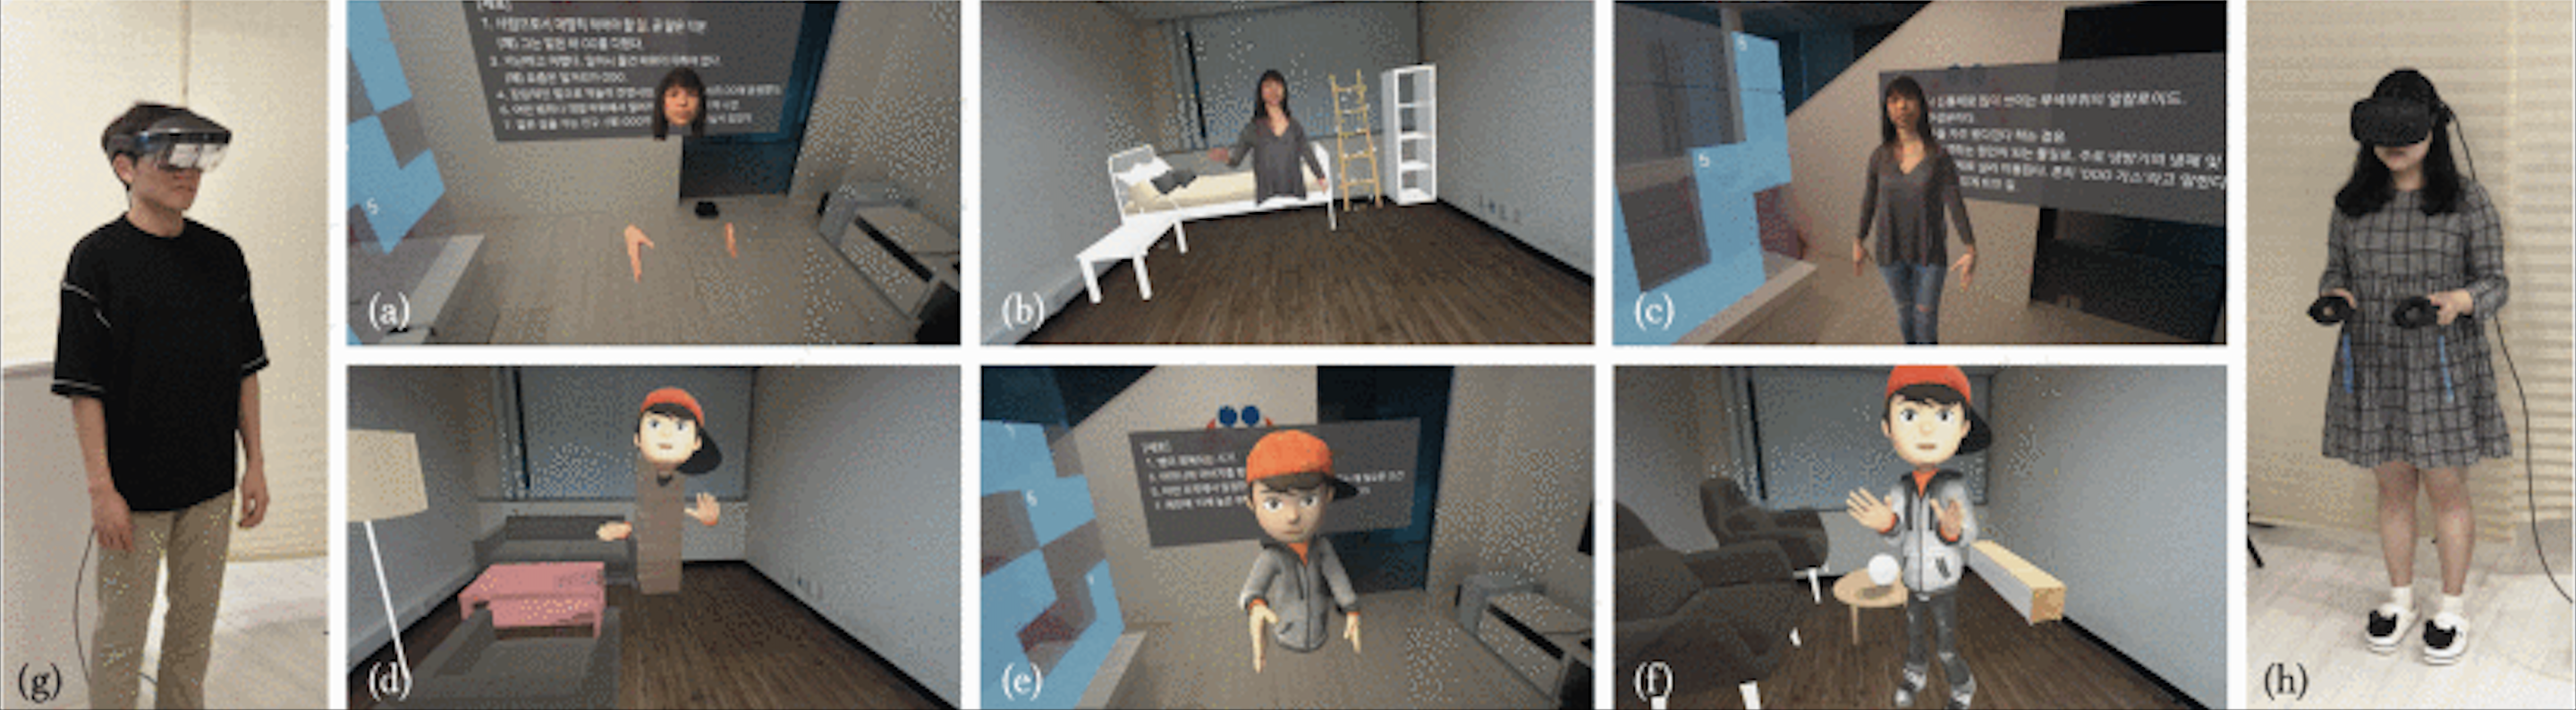
\includegraphics[width = 0.8\textwidth]{figures/Bildschirmfoto 2022-06-10 um 18.07.25}
\caption[Study 1 setup]{different avatar appearances}
\label{fig::avatarAppearences}
\end{figure}


The paper "The Effect of Avatar Appearance on Social Presence in an Augmented Reality Remote Collaboration" \cite{8797719}explores the effects some avatar design choices have on the user and how different visual representations of virtual agents will influence the social presence and user perception in an AR environment. To test this, a study was conducted, where 24 participants were asked to perform experimental tasks with an avatar, who was representing a remote collaborator, played by an actor. The avatar was displayed in one of six ways by changing the variables of Body part visibility and character style, which resulted in the following conditions: Realistic Whole Body (RWB), Realistic Upper Body (RUB), Realistic Head and Hands (RHH), Cartoon Whole Body (CWB), Cartoon Upper Body (CUB), Cartoon Head and Hands (CHH) as seen in Figure \ref{fig::avatarAppearences}.

\begin{figure}[H]
\centering
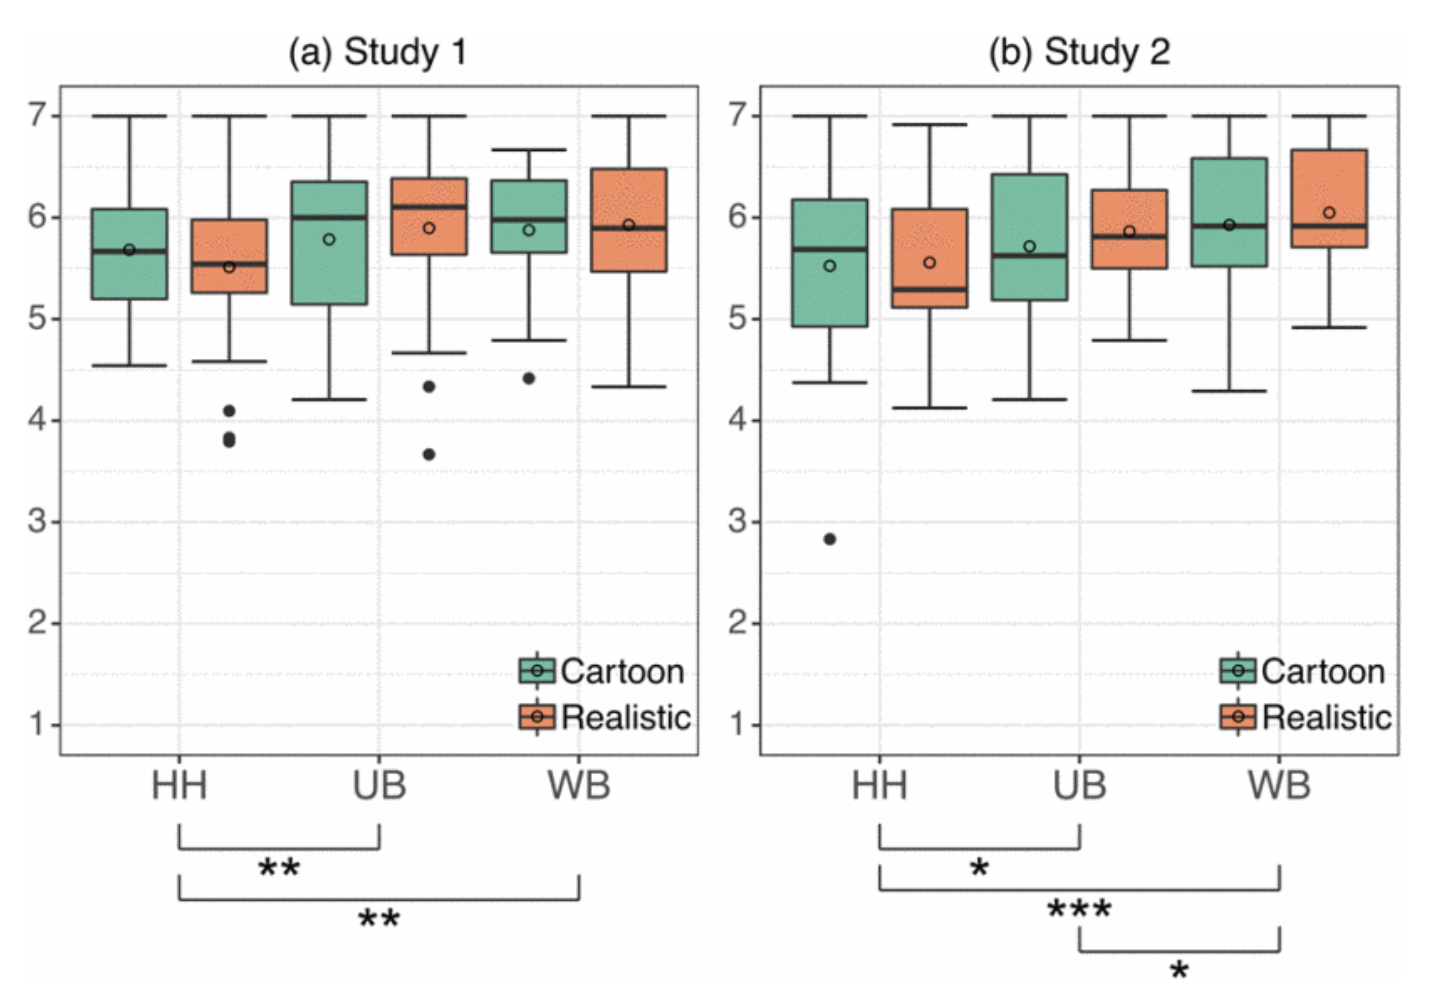
\includegraphics[width = 0.8\textwidth]{figures/Bildschirmfoto 2022-06-10 um 19.33.46}
\caption[Study 1 setup]{Aggregated social presence (1: Strongly disagree - 7: Strongly agree)}
\label{fig::avatarAppearences2}
\end{figure}


The study found that the Realistic Whole Body avatar was perceived as the most social present, with Cartoon Whole Body being a close second, and Head and Hands having the worst effect on the participants, both in cartoon and in realistic form as seen in \ref{fig::avatarAppearences2}.



\section{Social interaction in augmented reality}

The Paper “Social interaction in Augmented Reality” 
\cite{Carmigniani:2011te}
 focuses on the way augmented reality affects social interactions by creating three studies that mimick social situations with the addition of Augmented Reality, which infuses the situation with additional information. 

\subsection{Social inhibition and facilitation}
One interesting study was how the presence of virtual characters in the AR space influences people's task performance in the physical world. It is known that the presence of other people affects the task performance of humans, and it is a thoroughly studied theory in social psychology: social facilitation and inhibition. It refers to the fact that people tend to perform better in simple tasks when in the presence of other people, but on the other hand they perform worse on complex tasks. Zajonc’s drive theory can explain these tendencies: the presence of other people leads to an increase in one’s arousal, which in turn leads to better performance in simple tasks but a disadvantage in the execution of complex tasks.

\begin{figure}[H]
\centering
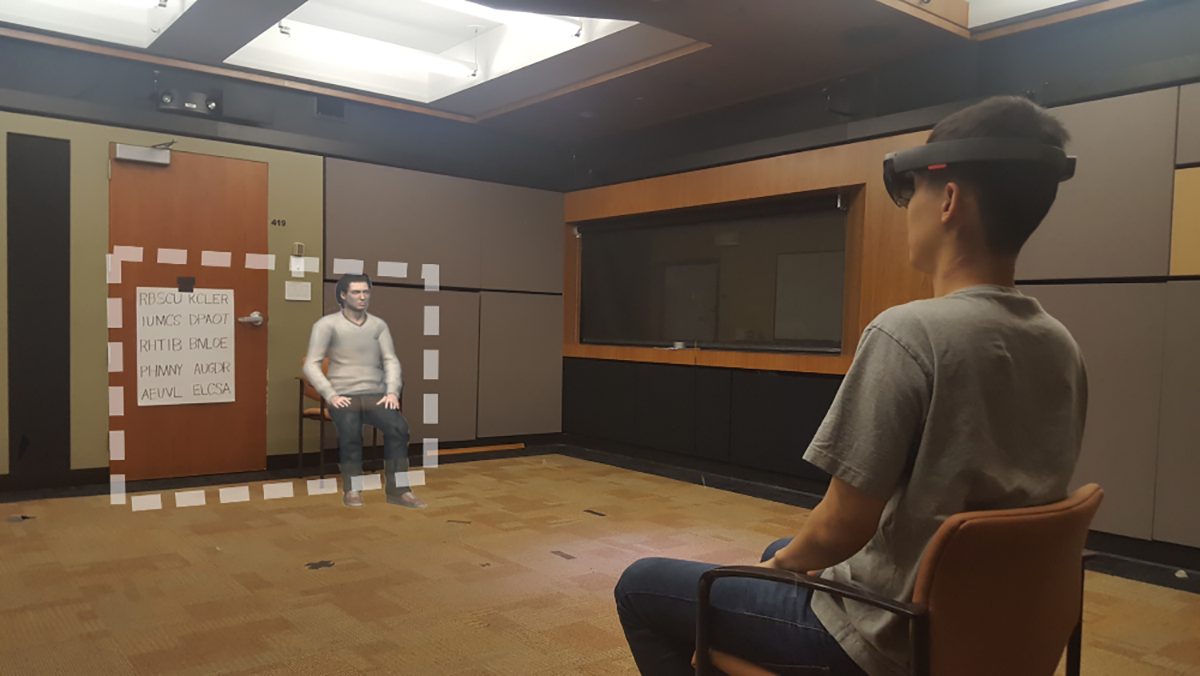
\includegraphics[width = 0.5\textwidth]{figures/pone.0216290.g001.PNG_L.png}
\caption[Study 1 setup]{This Figure shows the setup in which the study was conducted in}
\label{fig::firstSetup}
\end{figure}


This behavior has been tested and confirmed in Virtual Reality, but Miller’s paper focuses on these patterns in Augmented Reality. Due to the differences in surroundings and the presence of virtual characters instead of real humans, this behavior might be different in AR. To test this, they created a study recording the cognitive abilities of 60 participants by having them solve anagram tasks under the following conditions: Each participant was sitting alone in a 5.6 m by 6.4 m room equipped with a Microsoft HoloLens headset. A virtual agent would introduce himself, and the participant was informed that the agent would either stay during the completion of the task or leave the room, depending on the conditions, as shown in \ref{fig::firstSetup}. After that, the participants had three minutes to solve as many anagrams as they could, which were either hard or easy to solve, and read their answers out loud as soon as they solved them. This process was executed four times per participant, one time per combination of difficulty and social context. 


\begin{figure}[H]
\centering
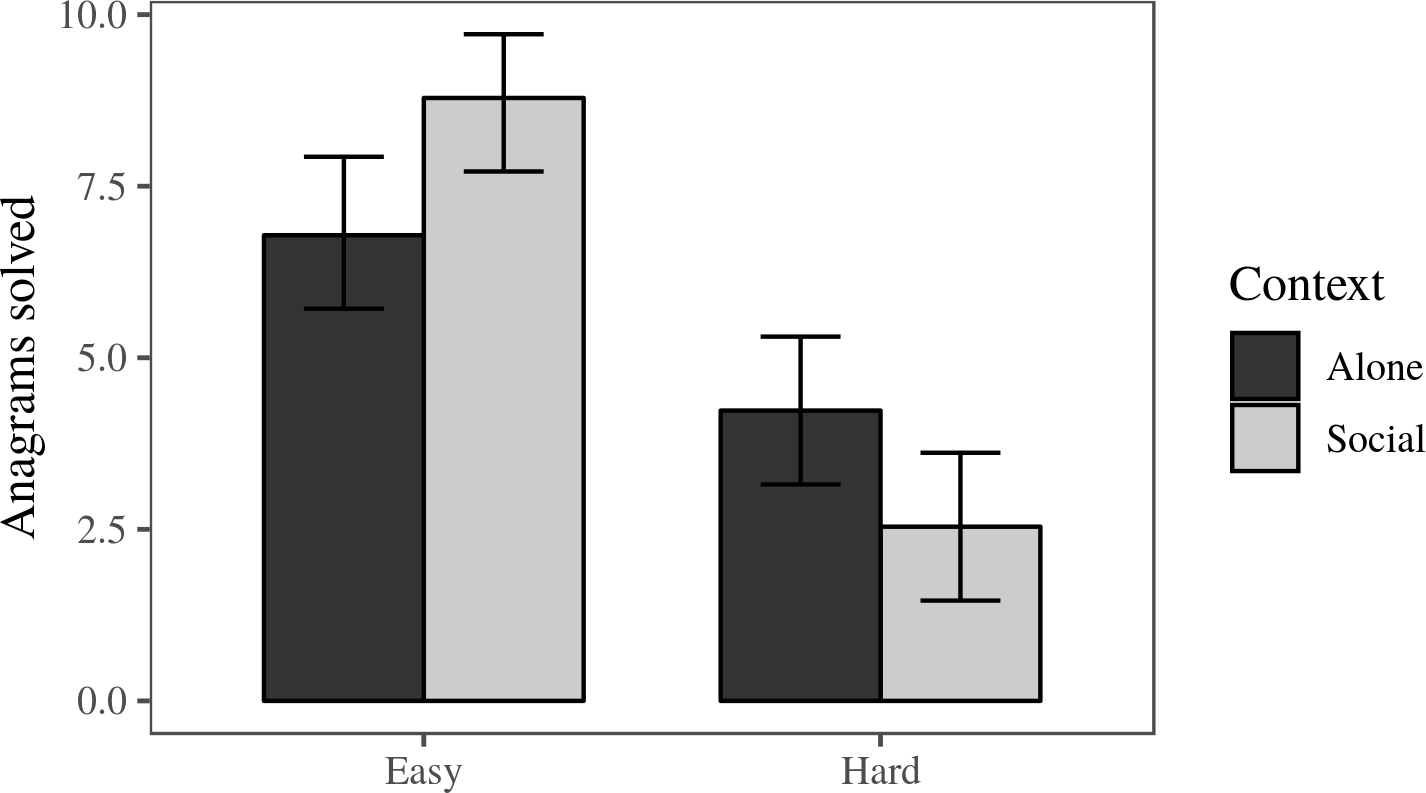
\includegraphics[width = 0.5\textwidth]{figures/pone.0216290.g003.PNG_L.png}
\caption[Study 1 result]{Results of the first study}
\label{fig::firstResult}
\end{figure}


Results showed that, like their physical counterparts, virtual agents indeed influence the performance of the participants as shown in \ref{fig::firstResult}. The participants performed significantly better at easy tasks with a virtual agent present while performing worse at harder tasks. With these results, it is clear that social facilitation and inhibition both exist even in Augmented reality with virtual agents.


One very interesting observation was how the participants improved their performance at the given tasks over time and how the effects of social facilitation and inhibition did not extend over multiple trials. This can be an indicator that the realism of the virtual agent is not high enough and that the participants get accustomed to the presence of the agent which in turn lowers the social pressure.

\subsection{Social norms in AR}

\begin{figure}[H]
\centering
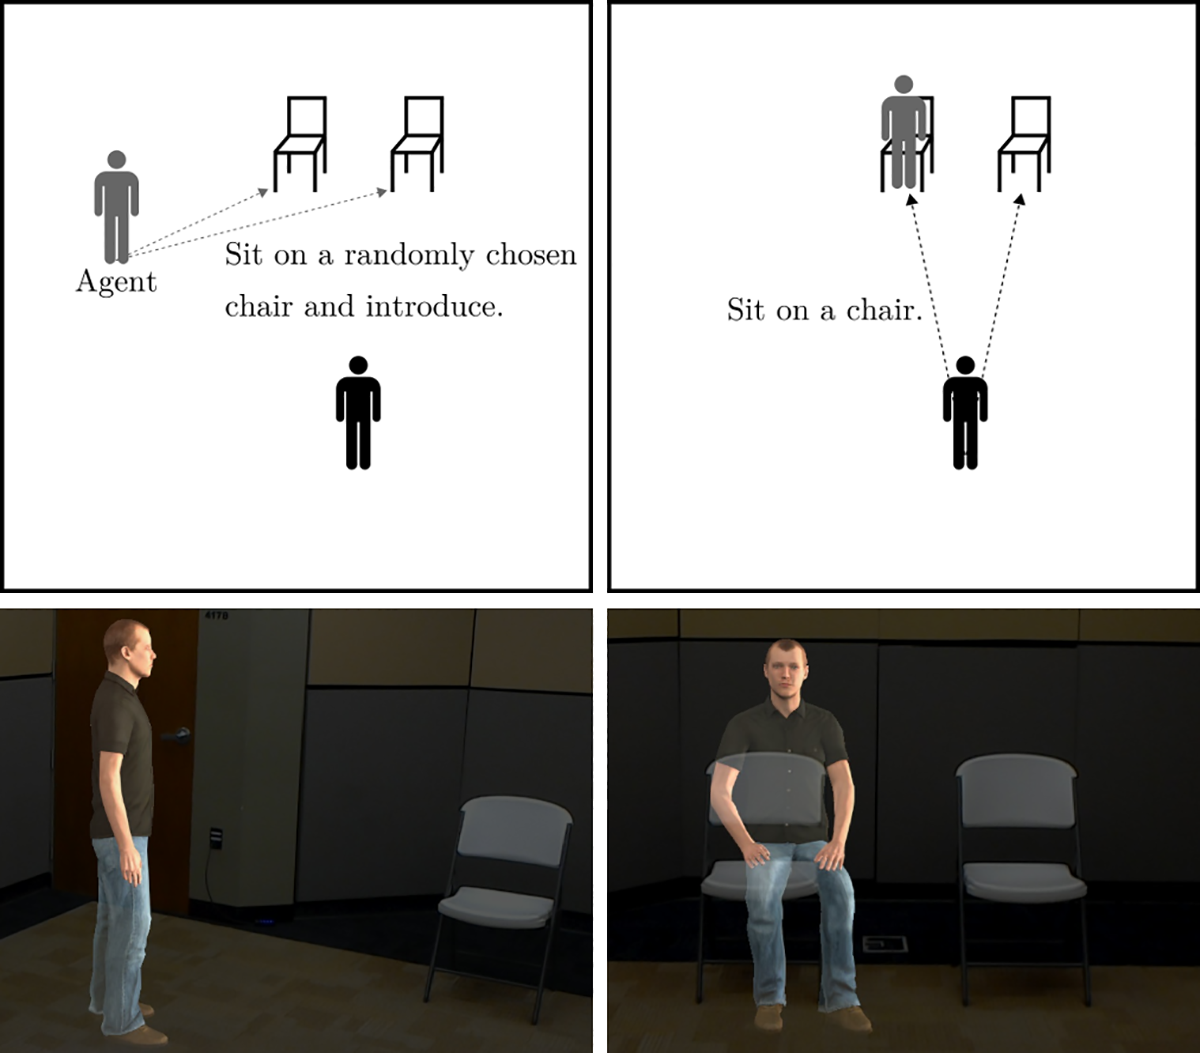
\includegraphics[width = 0.5\textwidth]{figures/pone.0216290.g004.PNG_L.png}
\caption[Study 1 result]{Setup of the second study}
\label{fig::secondStudy}
\end{figure}

In the second study of the paper, they tested if participants would adapt their nonverbal behavior including interpersonal distance and eye contact in the presence of a virtual agent. Additionally, they tested if the effect lasts even after taking the headset off. The procedure was the following: The participants were randomly assigned one of two conditions, either "Headset" or "without Headset". Under both conditions, the participants started with a headset and saw a virtual agent walk across the room and sit down in one of two chairs as shown in \ref{fig::secondStudy}. After that, only the participants with the "without Headset" conditions took off their Headset and the participant was asked to sit on one of the two chairs. 

After conducting the study, it was clear that the participants wearing the Headset avoided sitting on the agent, and the participants without the headset were still significantly more likely to sit on the chair without the agent, even without seeing him.
\subsection{Social connectedness between AR users and non-users}

The goal of the last study of the paper was to test if the social connectedness between people suffers if one person is wearing an AR headset. To test this, two random participants were put in a small room, with one participant wearing an AR headset and the other one not. There were two possible conditions: in the virtually occluded condition, there was a logo superimposed onto the other participant, in the not virtually occluded condition the logo was next to the partner. Then, the participants were asked to discuss something interesting that happened to them in the past month for 5 minutes, and afterward, they both completed a questionnaire about the experience where they ranked their social connectedness from 1 to 5.

The results showed that there was no significant difference in the social connectedness, interpersonal attraction, and social presence between virtually occluded and not virtually occluded users. However, regardless of condition, AR users tend to have a lower social presence, connectedness, and interpersonal attraction than the person not using the headset.

\section{Collaborative Augmented Reality}

This paper explores the collaborative aspect of AR and how it can be used to improve face-to-face and remote collaboration \cite{CollaborativeAR}. AR offers many benefits, like seamless interaction between real and virtual environments and the ability to enhance reality, which is really useful when collaborating. In this paper, collaboration gets split into two categories: remote collaboration and face-to-face collaboration. in both cases, AR offers many benefits.

\subsection{face-to-face collaboration}
For face-to-face collaboration, when discussing virtual objects, many non-verbal cues get lost. For example, discussing an object on the screen can be frustrating because there is no way to reference on-screen objects with the precision and intuition of real objects. Augmented Reality can be used to project onto and enhance the physical workspace for face-to-face collaboration and improve the efficiency of these kinds of collaborations by making them very intuitive, even when rendering 3D models.

\begin{figure}[H]
\centering
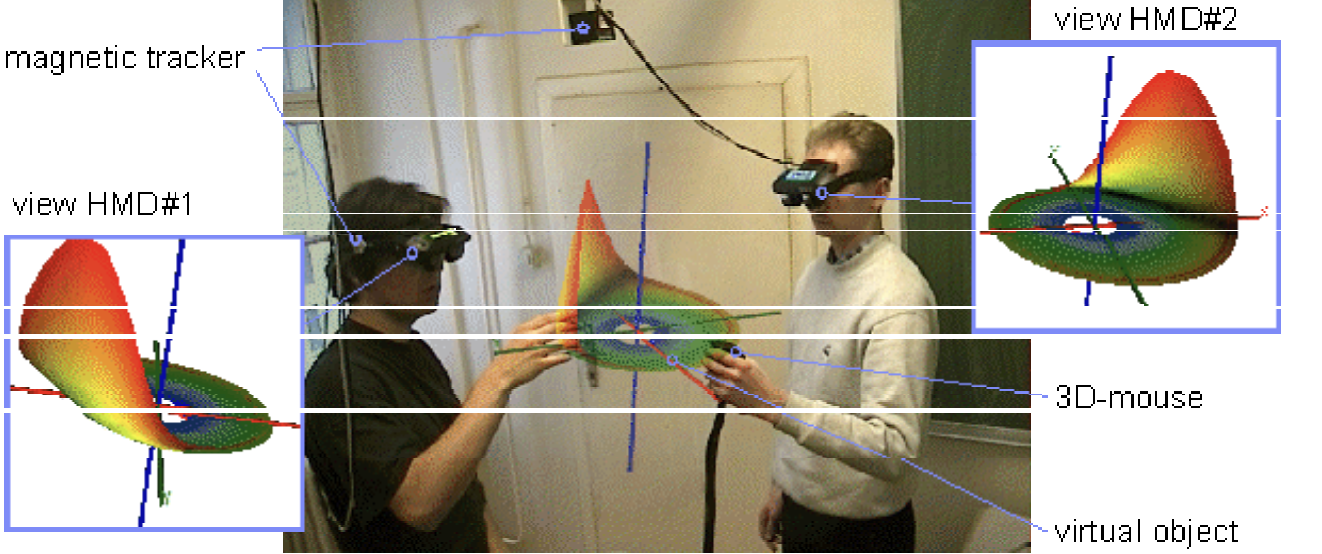
\includegraphics[width = 0.5\textwidth]{figures/Bildschirmfoto 2022-06-10 um 18.47.26}
\caption[Study 1 setup]{This Figure shows the StudierStube AR interface}
\label{fig::StudierStube}
\end{figure}

 A study at StudierTube by Schmalsteig et. al. \cite{studierstube} tried out face-to-face collaborations by having two participants wear see-through head-mounted displays and collaboratively view a 3d-object superimposed onto the real environment. By reporting this process they found these main benefits for collaborative AR environments:

\begin{itemize}
\item Virtuality: Objects that don’t exist in the real world can be viewed and examined. 
\item  Augmentation: Real objects can be augmented by virtual annotations. 
\item  Cooperation: Multiple users can see each other and cooperate in a natural way. 
\item Independence: Each user controls his own independent viewpoint.
\item Individuality: Displayed data can be different for each viewer.
\end{itemize}

Additional studies by Billinghurst et al. explored the benefits of AR collaboration by comparing the approach to problem-solving in face-to-face collaborations with real objects, co-located AR collaboration with virtual objects, and co-located projection screen-based collaboration with virtual objects. The results showed that speech and gesture behaviors in face-to-face and AR problem solving were very similar, which underlines the improved intuition with AR collaboration. However, the participants still felt that face-to-face conditions and AR were not similar, which can be attributed to the use of relatively old technology from 2002, so there is room for additional studies that test this with newer equipment.

\subsection{Remote collaboration}

In remote collaboration, AR has many applications as well. A user study by Billinghurst et al. found that AR video conferencing gave the participants a "significantly higher sense of presence" and that made it easier for participants to pick up on non-verbal cues, which are very important for high social presence. This paper, even while being from the Year 2002 when the AR technology was still very limited, saw big potential in AR remote conferencing.
